\documentclass[12pt]{article}
\usepackage[margin=1in]{geometry}
\usepackage{mdframed}
\usepackage{booktabs}

% For math
\usepackage{amsmath, amsthm, amssymb}

% For coding
\usepackage{listings}
\lstset{ %
  frame=single,
  numbers=left,
  backgroundcolor=\color{white},   % choose the background color
  basicstyle=\footnotesize,        % size of fonts used for the code
  breaklines=true,                 % automatic line breaking only at whitespace
  captionpos=b,                    % sets the caption-position to bottom
  commentstyle=\color{mygreen},    % comment style
  escapeinside={(*@}{@*)},         % if you want to add LaTeX within your code
  keywordstyle=\color{blue},       % keyword style
  stringstyle=\color{mymauve},     % string literal style
  tabsize=1,
}

% For SI numerical display.
\usepackage{siunitx}
\sisetup{detect-all}

% For tikz pictures
\usepackage{tikz}
\usepackage{pgfplots}

% For table \*rules
\usepackage{booktabs}

% To fix table places.
\usepackage{float}

% For autoref
\usepackage{hyperref}

\restylefloat{table}

\title{ECS 230 App Num Linear Algebra \\ Homework 2}
\author{Yuyang(Peter) Rong \\917781535 \\ PtrRong@ucdavis.edu}

\begin{document}

\maketitle

\section{Simple Matrix Multiplication}
Write a program that implements matrix multiplication $C=AB$ where $A$, $B$ and $C$ are $\mathbb{R}^{(n \times n)}$ real matrices represented as double-precision numbers.

a) Provide results for the following values of n: 100 200 500 1000 2000

b) Comment on your results and compare with the expected floating-point performance of
the processor (Intel Core i7-4790K, 4.0 GHz or 3.6 GHz depending on the CSIF PC you are
using. Note: determine the peak performance of one core of the processor considering the
width of SIMD registers, clock frequency, hyperthreading, and the fused multiply-add FMA
instruction). Compute the fraction of the nominal peak performance of a core achieved in
your runs. Consider the fact that the “turbo boost” feature of Intel processors may change
the frequency.



\subsection{Running results}

\subsubsection{Running the Program}
For simplicity we used \texttt{Makefile} to make all our projects.
You may find the whole file in the attachment \autoref{sec:makefile}.
Here is the part corresponding to this problem.
\begin{lstlisting}
mul: $(SRC)/mul.c
  gcc $^ -o $(TARGET)/$@
        \end{lstlisting}

Shell script:
\begin{lstlisting}
for i in 100 200 500 1000 2000
do
    for j in 1 2 3
    do
        echo "Running \`mul $i\` for the $j-th time"
        ./target/mul $i >/dev/null
    done
done
\end{lstlisting}

\begin{table}[H]
  \centering
  \begin{tabular}{lrrrr}
    \toprule
    n                           &
    \multicolumn{1}{l}{Trial 1} &
    \multicolumn{1}{l}{Trial 2} &
    \multicolumn{1}{l}{Trial 3} &
    \multicolumn{1}{l}{Avg clocks}                                                          \\
    \midrule
    100                         & 12649539     & 12863349     & 12625674     & 12712854     \\
    200                         & 109423755    & 109387578    & 108833259    & 109214864    \\
    500                         & 1948191642   & 1955382339   & 1955747193   & 1953107058   \\
    1000                        & 23103685602  & 22953968622  & 33171786723  & 26409813649  \\
    2000                        & 273302156799 & 277051750074 & 282126904803 & 277493603892 \\
    \bottomrule
  \end{tabular}
  \caption{Results of running program 3 times}
\end{table}


\subsubsection{Formulas}
Since we are running on \texttt{Intel(R) Xeon(R) Silver 4116 CPU @ 2.10GHz},
CPU frequency is a fixed number $f = 2101 \si{\MHz}$
after querying \lstinline{\proc\cpuinfo}
\begin{equation}
  \begin{aligned}
    % Total number of floating point operation
    \text{gflops}   & = 2n^3                                                             \\
    % Time taken to compute the product                         
    \text{time}     & = \frac{\text{cycles}}{f}                                          \\
    % Floating point performance GFlops/s
    \text{gflops/s} & = \frac{\text{gflops}}{\text{time}} = \frac{2n^3 f}{\text{cycles}}
  \end{aligned}
\end{equation}

\begin{table}[H]
  \centering
  \begin{tabular}{lrr}
    \toprule
    \multicolumn{1}{l}{n}            &
    \multicolumn{1}{l}{Clock cycles} &
    \multicolumn{1}{l}{Gflops/s}                               \\
    \midrule
    100                              & 12712854     & 0.566356 \\
    200                              & 109214864    & 0.527401 \\
    500                              & 1953107058   & 0.460804 \\
    1000                             & 26409813649  & 0.272626 \\
    2000                             & 277493603892 & 0.207572 \\
    \bottomrule
  \end{tabular}
  \caption{Results of running program in subsection a}
\end{table}

\begin{figure}[t]
  \centering
  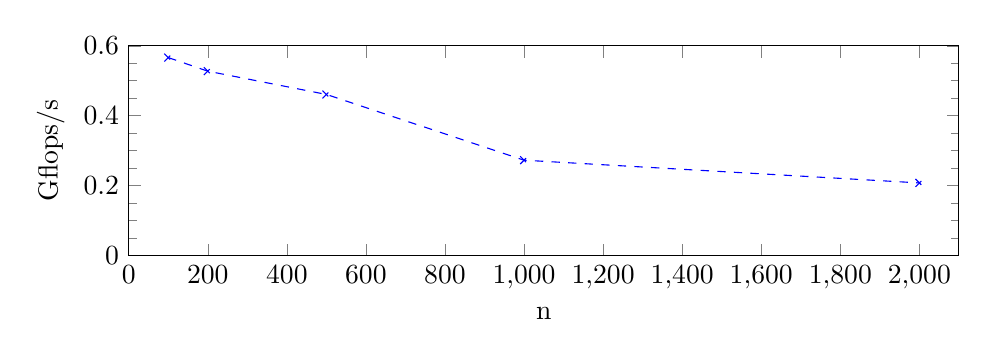
\begin{tikzpicture}
    \begin{axis}[
        ymin=0, ymax=0.6,
        xmin=0, xmax=2100,
        width=\linewidth,
        height=0.35\linewidth,
        xlabel={n},
        ylabel={Gflops/s},
        minor y tick num =3,
        legend pos=south west
      ]
      \addplot +[dashed, mark=x] plot coordinates {
          (100 , 0.566356)
          (200 , 0.527401)
          (500 , 0.460804)
          (1000 , 0.272626)
          (2000 , 0.207572)
        };
    \end{axis}
  \end{tikzpicture}
  \caption{Gflops/s change over matrix dimension change}
\end{figure}

\subsection{Analysis}
\subsubsection{Peak performance}
\begin{equation}
  \begin{aligned}
    \text{peak} & = f * \frac{\text{SIMD width}}{\text{8 * sizeof(double)}}\text{flop} * \text{hyperthreading} * \text{FMA} \\
                & = 2101 \si{MHz} * \frac{256}{64}\text{ flops} * 2 * 2                                                     \\
                & = 33.616 \text{ Gflops/s}
  \end{aligned}
\end{equation}

\subsubsection{Why we didn't reach peak}

The main reason is that CPU need to wait for the data to be featched from memory.
Generally, fetch is generally takes 100~1000 CPU cycles, which would slow the program down by at least 100x.

\section{Matrix Multiplication Loops}
Write a modified version of the above program implementing all 6 possible loop orderings in a matrix multiplication.
Run the program and compare the performance for each loop ordering. Discuss and explain your results.  Compare results obtained when compiling with \lstinline$gcc$ without options, and with the \lstinline$-O0$,\lstinline$-O2$ and \lstinline$-O3$ optimization options.

\subsection{Results}

\subsubsection{Running the Program}
For simplicity we used \texttt{Makefile} to make all our projects.
You may find the whole file in the attachment \autoref{sec:makefile}.
Here is the part corresponding to this problem.
\begin{lstlisting}
mul_loop_%: $(SRC)/mul_loop.c
  gcc $^ -$* -DOPT_LEVEL=\"-$*\" -o $(TARGET)/$@
\end{lstlisting}

Shell script:
\begin{lstlisting}
run_mul_loop () { 
    for j in 1 2 3
    do
        echo "Running \`mul_loop 1000\` for the $j-th time"
        ./target/mul_loop_$1 1000 >/dev/null
    done
}

run_mul_loop O0
run_mul_loop O2
run_mul_loop O3
\end{lstlisting}

\subsubsection{Algorithms}

\begin{lstlisting}[language=C]
typedef size_t usize;
typedef double Real;

typedef struct {
  Real* ptr;
  usize n;
} Matrix;

#define I for (usize i = 0; i < n; i++)
#define J for (usize j = 0; j < n; j++)
#define K for (usize k = 0; k < n; k++)

#define MATRIX_GET(m, i, j) (m.ptr + i * m.n + j)
#define MATRIX_MUL(a, b, c) \
  *MATRIX_GET(a, i, j) = *MATRIX_GET(b, i, k) * *MATRIX_GET(c, k, j)

I J K { MATRIX_MUL(a, b, c); }
I K J { MATRIX_MUL(a, b, c); }
J I K { MATRIX_MUL(a, b, c); }
J K I { MATRIX_MUL(a, b, c); }
K I J { MATRIX_MUL(a, b, c); }
K J I { MATRIX_MUL(a, b, c); }
\end{lstlisting}

Here, we run the program with argument 1000.
Notice that when no optimization option is given to \lstinline{gcc} it acts as if \lstinline{-O0} is given.
So we didn't do experiment on binary compiled with no optimization level.

\begin{table}[H]
  \centering
  \begin{tabular}{lrrrr}
    \toprule
    \multicolumn{1}{l}{Loop Order} &
    \multicolumn{1}{l}{Trial 1}    &
    \multicolumn{1}{l}{Trial 2}    &
    \multicolumn{1}{l}{Trial 3}    &
    \multicolumn{1}{l}{Avg Gflops}                                             \\
    \midrule
    ijk                            & 0.334930 & 0.337002 & 0.303872 & 0.325268 \\
    ikj                            & 0.638082 & 0.637957 & 0.628563 & 0.634867 \\
    jik                            & 0.467406 & 0.465052 & 0.457110 & 0.463189 \\
    jki                            & 0.152060 & 0.144394 & 0.147171 & 0.147875 \\
    kij                            & 0.628118 & 0.616514 & 0.611908 & 0.618847 \\
    kji                            & 0.154302 & 0.150236 & 0.149007 & 0.151182 \\
    \bottomrule
  \end{tabular}
  \caption{Gflops of running different loops for 3 times using argument $1000$ under \lstinline{O0}}
\end{table}
\begin{table}[H]
  \centering
  \begin{tabular}{lrrrr}
    \toprule
    \multicolumn{1}{l}{Loop Order} &
    \multicolumn{1}{l}{Trial 1}    &
    \multicolumn{1}{l}{Trial 2}    &
    \multicolumn{1}{l}{Trial 3}    &
    \multicolumn{1}{l}{Avg Gflops}                                             \\
    \midrule
    ijk                            & 1.090042 & 1.128116 & 1.098015 & 1.105391 \\
    ikj                            & 3.206651 & 3.475044 & 3.238233 & 3.306643 \\
    jik                            & 1.506337 & 1.501654 & 1.518204 & 1.508732 \\
    jki                            & 0.149234 & 0.148623 & 0.149306 & 0.149054 \\
    kij                            & 2.801252 & 2.906616 & 2.763490 & 2.823786 \\
    kji                            & 0.149279 & 0.148460 & 0.148870 & 0.148870 \\
    \bottomrule
  \end{tabular}
  \caption{Gflops of running different loops for 3 times using argument $1000$ under \lstinline{O2}}
\end{table}
\begin{table}[H]
  \centering
  \begin{tabular}{lrrrr}
    \toprule
    \multicolumn{1}{l}{Loop Order} &
    \multicolumn{1}{l}{Trial 1}    &
    \multicolumn{1}{l}{Trial 2}    &
    \multicolumn{1}{l}{Trial 3}    &
    \multicolumn{1}{l}{Avg Gflops}                                             \\
    \midrule
    ijk                            & 1.093538 & 1.093790 & 1.107969 & 1.098432 \\
    ikj                            & 4.319633 & 4.285197 & 4.325042 & 4.309957 \\
    jik                            & 1.520591 & 1.529733 & 1.521390 & 1.523905 \\
    jki                            & 0.149253 & 0.149589 & 0.148259 & 0.149034 \\
    kij                            & 3.485271 & 3.498210 & 3.345640 & 3.443040 \\
    kji                            & 0.148638 & 0.149443 & 0.150526 & 0.149536 \\
    \bottomrule
  \end{tabular}
  \caption{Gflops of running different loops for 3 times using argument $1000$ under \lstinline{O3}}
\end{table}

\begin{table}[H]
  \centering
  \begin{tabular}{lSSS}
    \toprule
    \multicolumn{1}{l}{Loop Order} &
    \multicolumn{1}{l}{-O0 avg}    &
    \multicolumn{1}{l}{-O2 avg}    &
    \multicolumn{1}{l}{-O3 avg}                                     \\
    \midrule
    ijk                            & 0.325268 & 1.105391 & 1.098432 \\
    ikj                            & 0.634867 & 3.306643 & 4.309957 \\
    jik                            & 0.463189 & 1.508732 & 1.523905 \\
    jki                            & 0.147875 & 0.149054 & 0.149034 \\
    kij                            & 0.618847 & 2.823786 & 3.443040 \\
    kji                            & 0.151182 & 0.148870 & 0.149536 \\
    \bottomrule
  \end{tabular}
  \caption{Results of running different loops}
\end{table}


\begin{figure}[t]
  \centering
  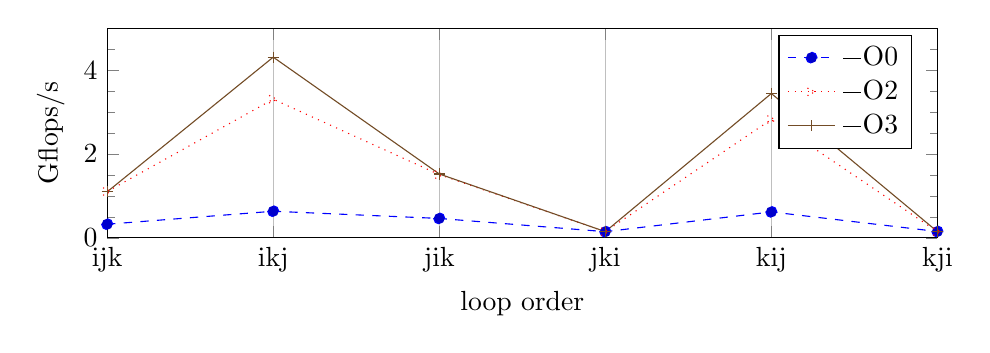
\begin{tikzpicture}
    \begin{axis}[
        ymin=0, ymax=5,
        xtick=data,
        xmajorgrids,
        xticklabels={
            ijk,
            ikj,
            jik,
            jki,
            kij,
            kji},
        xmin=1, xmax=6,
        width=\linewidth,
        height=0.35\linewidth,
        xlabel={loop order},
        ylabel={Gflops/s},
        minor y tick num =3,
        legend pos=north east
      ]
      \addplot +[dashed, mark=*] plot coordinates {
          (1 , 0.325268)
          (2 , 0.634867)
          (3 , 0.463189)
          (4 , 0.147875)
          (5 , 0.618847)
          (6 , 0.151182)
        };
      \addplot +[dotted, mark=x] plot coordinates {
          (1 , 1.105391)
          (2 , 3.306643)
          (3 , 1.508732)
          (4 , 0.149054)
          (5 , 2.823786)
          (6 , 0.148870)
        };
      \addplot +[mark=+] plot coordinates {
          (1 , 1.098432)
          (2 , 4.309957)
          (3 , 1.523905)
          (4 , 0.149034)
          (5 , 3.443040)
          (6 , 0.149536)
        };
      \legend{\lstinline{-O0} \\\lstinline{-O2} \\\lstinline{-O3} \\}
    \end{axis}
  \end{tikzpicture}
  \caption{Gflops/s change over loop order change.}
\end{figure}

\section{BLAS Matrix Multiplication}
Write a program implementing matrix multiplication using the  \lstinline$dgemm$ function of the BLAS library(http://www.netlib.org/blas). The library is installed on CSIF computers.  Use the command  \lstinline$man dgemm$ on CSIF to get details about the arguments of the function. Note that  \lstinline$dgemm$ is a FORTRAN function and all parameters from a C program should be passed through pointers. Use the \textit{dotblas.c} example program (provided on Canvas) as an example of how to call BLAS functions. Use the additional \lstinline$-lblas$ argument during compilation.

\textbf{Measure timings for the above problem sizes and discuss your results.}

Note: all programs in this homework assignment use only one core of the processor. However, the BLAS library is multithreaded.
Use the command \lstinline$export OMP_NUM_THREADS=1$ before running your program to make sure that you measure the performance of one core only

\textbf{Solutions}


\textbf{Results of running different loops}

\begin{table}
  \centering
  \begin{tabular}{SSS}
    \toprule
    \multicolumn{1}{l}{\lstinline{dgemm} dimension} &
    \multicolumn{1}{l}{Clock cycle}                 &
    \multicolumn{1}{l}{Total seconds}                     \\
    \midrule
    100                                             &   & \\
    200                                             &   & \\
    500                                             &   & \\
    1000                                            &   & \\
    2000                                            &   & \\
    \bottomrule
  \end{tabular}
  \caption{Some caption}

\end{table}



\begin{figure}
  \centering
  \fbox{\rule[-.5cm]{0cm}{4cm} \rule[-.5cm]{4cm}{0cm}}
  \caption{Replace fbox with your graph.  X axis is for different dimension and Y for clock cycle}
\end{figure}


\textbf{Running the Program}

\begin{mdframed}
  % TODO
  Compilation: \lstinline$gcc -o output filename.c -flags$

  Running: \lstinline$./output n$

\end{mdframed}

\textbf{Formula}

\begin{mdframed}
  $$\text{total\_seconds} = $$
\end{mdframed}

\textbf{Discussing the Results}

\begin{mdframed}
  \vspace{3em}

\end{mdframed}

\appendix

\section{Makefile}
\label{sec:makefile}
\begin{lstlisting}
SRC=src
TARGET=target

.PHONY: all

all: mul mul_loop_O0 mul_loop_O2 mul_loop_O3 mul_BLAS

mul: $(SRC)/mul.c
  gcc $^ -o $(TARGET)/$@

mul_loop_%: $(SRC)/mul_loop.c
gcc $^ -$* -DOPT_LEVEL=\"-$*\" -o $(TARGET)/$@

  mul_BLAS: $(SRC)/mul_BLAS.c
gcc $^ -o $(TARGET)/$@ -lblas

  clean:
  rm $(TARGET)/mul*
\end{lstlisting}

\end{document}